\section{File Systems}

\paragraph{File Systems --- Motivation}
\begin{itemize}
  \item \textbf{Goal}: enable storing of large data amounts
  \begin{itemize}
    \item store data/program consistently + persistently
    \item easily look up previously stored data/program
  \end{itemize}
  \item \textbf{File types}:
  \begin{itemize}
    \item \emph{data} (numeric, character, binary)
    \item \emph{program}
  \end{itemize}
\end{itemize}

\paragraph{File Systems --- Overview}
\begin{itemize}
  \item OS may support multiple file systems
  \item \textbf{Namespace}: all file systems typically bound into single namespace (often hierarchical, rooted tree)
\end{itemize}

\paragraph{Files -- Abstract operations}
\begin{itemize}
  \item \textbf{File}: abstract data type/object, offering
  \begin{itemize}
    \item \code{create}, \code{write}, \code{read},
    \item \code{reposition} (within file),
    \item \code{delete}, \code{truncate},
    \item \code{open(}$ F_i $\code{)} (search directory structure on disk for entry $ F_i $, move meta data to memory),
    \item \code{close(}$ F_i $\code{)} (move cached meta data of entry $ F_i $ in memory to directory structure on disk)
  \end{itemize}
\end{itemize}
\begin{figure}[h]\centering\label{FileSystemInteraction}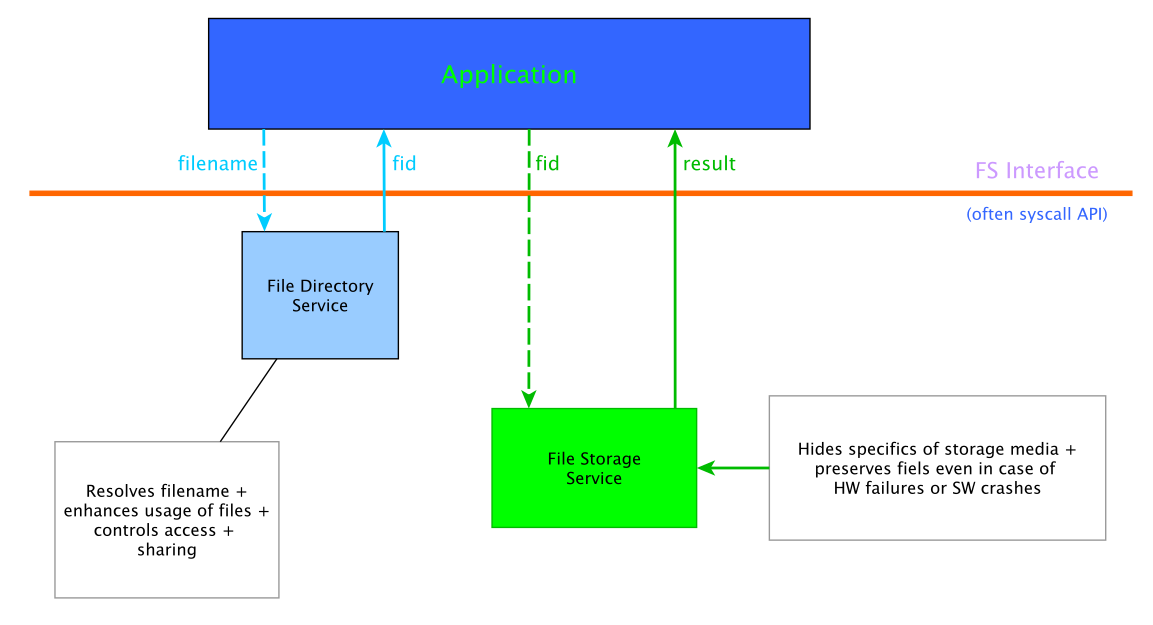
\includegraphics[width=0.4\textwidth]{FileSystemInteraction}\end{figure}

\paragraph{File Management --- Goals}
\begin{itemize}
  \item provide convenient file naming scheme
  \item provide uniform I/O support for variety of storage device types
  \item provide standardized set of I/O interface functions
  \item minimize/eliminate loss/corruption of data
  \item provide I/O support + access control for multiple users
  \item enhance system administration (e.g., backup)
  \item provide acceptable performance
\end{itemize}

\paragraph{File Management --- Open files}
\begin{itemize}
  \item several meta data is needed to manage open files
  \item \textbf{File pointer}: pointer to last read/write location, per process that has file opened
  \item \textbf{Access rights}: per-process access mode information
  \item \textbf{File-open count}: counter of number of times a file is opened (to allow removal of data from open-file table when last process closes)
  \item \textbf{Disk location}: cache of data access information
\end{itemize}

\paragraph{File Access}
\begin{itemize}
  \item \textbf{Strictly sequential} (early systems):
  \begin{itemize}
    \item read all bytes/records from beginning
    \item cannot jump round, could only rewind
    \item sufficient as long as storage was a tape
  \end{itemize}
  \item \textbf{Random access} (current systems):
  \begin{itemize}
    \item bytes/records read in any order
    \item essential for database systems
  \end{itemize}
\end{itemize}

\paragraph{Directories --- Goals}
\begin{itemize}
  \item \textbf{Naming}: convenient to users
  \begin{itemize}
    \item two users can have same name for different files
    \item same file can have several different names
  \end{itemize}
  \item \textbf{Grouping}: logical grouping of files by properties
  \item \textbf{Efficiency}: fast operations
\end{itemize}

\paragraph{Files --- Sharing}
\begin{itemize}
  \item \textbf{Issues}:
  \begin{itemize}
    \item efficiently access to same file?
    \item how to determine access rights?
    \item management of concurrent accesses?
  \end{itemize}
  \item \textbf{Access rights}:
  \begin{itemize}
    \item \emph{none}: existence unknown to user, user cannot read directory containing file 
    \item \emph{knowledge}: user can only determine existence and file ownership 
    \item \emph{execution}: user can load + execute program, but can not copy it 
    \item \emph{reading}: user can read file (includes copying + execution) 
    \item \emph{appending}: user can only add data to file, but cannot modify/delete data in file 
    \item \emph{updating}: user can modify + delete + add to file (includes creating + removing all data) 
    \item \emph{change protection}: user can change access rights granted to other users 
    \item \emph{deletion}: user can delete file 
    \item \emph{owner}: all previous rights + rights granting
  \end{itemize} 
  \item \textbf{Concurrent access}:
  \begin{itemize}
    \item \emph{application locking}: application can lock entire file or individual records for updating 
    \item \emph{exclusive vs. shared}: writer lock vs. multiple readers allowed 
    \item \emph{mandatory vs. advisory}: access denied depending on locks vs. process can decide what to do
  \end{itemize}
\end{itemize}